%\documentclass[handout]{beamer}
\documentclass{beamer}
%\usepackage{beamerarticle}
\usepackage{tikz}
\usetikzlibrary{arrows,shapes}
\usepackage{heppennames}
\usepackage{hepnicenames}
\usepackage{listings}
\newcommand{\whizard}{WHIZARD\xspace}

\author{S. Poss for the PH-LCD group}
\title{Use of \whizard for the mass production of CLIC CDR volume 2}
%\subtitle{Update}
\institute[CERN]
{
  CERN
}
\date{November 22nd, 2011}
\mode<presentation>
{
   \setbeamertemplate{navigation symbols}{}
   \setbeamertemplate{footline}[frame number] 
}

\AtBeginSection[]
{
\begin{frame}<beamer>
\frametitle{Outline}
\tableofcontents[currentsection,currentsubsection]
\end{frame}
}


\begin{document}
\begin{frame}
\titlepage
\end{frame}
\begin{frame}
\frametitle{Outline}
\tableofcontents
% You might wish to add the option [pausesections]
\end{frame}
\tikzstyle{decision} = [diamond, draw, text badly centered, node distance=2.8cm]
\tikzstyle{block} = [rectangle, draw, text centered, rounded corners, text width=1.9cm, node distance=2.2cm]
\tikzstyle{autoblock} = [rectangle, draw, text centered, rounded corners, node distance=2.2cm]
\tikzstyle{line} = [draw, -triangle 90]
\tikzstyle{dline} = [draw, dashed, -triangle 90]
%\tikzstyle{cloud} = [draw, ellipse,fill=red!20, node distance=3cm,minimum height=2em]
\section{Introduction}

\begin{frame}
\frametitle{Introduction}
CLIC detector studies use ILC concepts as baseline: \alert{use common tools}.\\
For generation, linear collider common generator tools group:\\
use \whizard1.95 as proved to be good for ILC LOIs.\\
~\\
CLIC detector studies as presented in the Conceptual Design Report (CDR):
study 6 physics channels to assess detector performance.\\
~\\
This presentation:
\begin{itemize}
  \item Channels studied
  \item Tools developed for mass production
  \item Limitations
\end{itemize}
\end{frame}

\begin{frame}
\frametitle{A short word on CLIC}
CLIC is
\begin{itemize}
  \item an $\Pep\Pem$ linear collider
  \item operating nominally at 3TeV cme
  \item 2 detector concepts (ILD and SiD) based on ILC concepts
\end{itemize}
\begin{center}
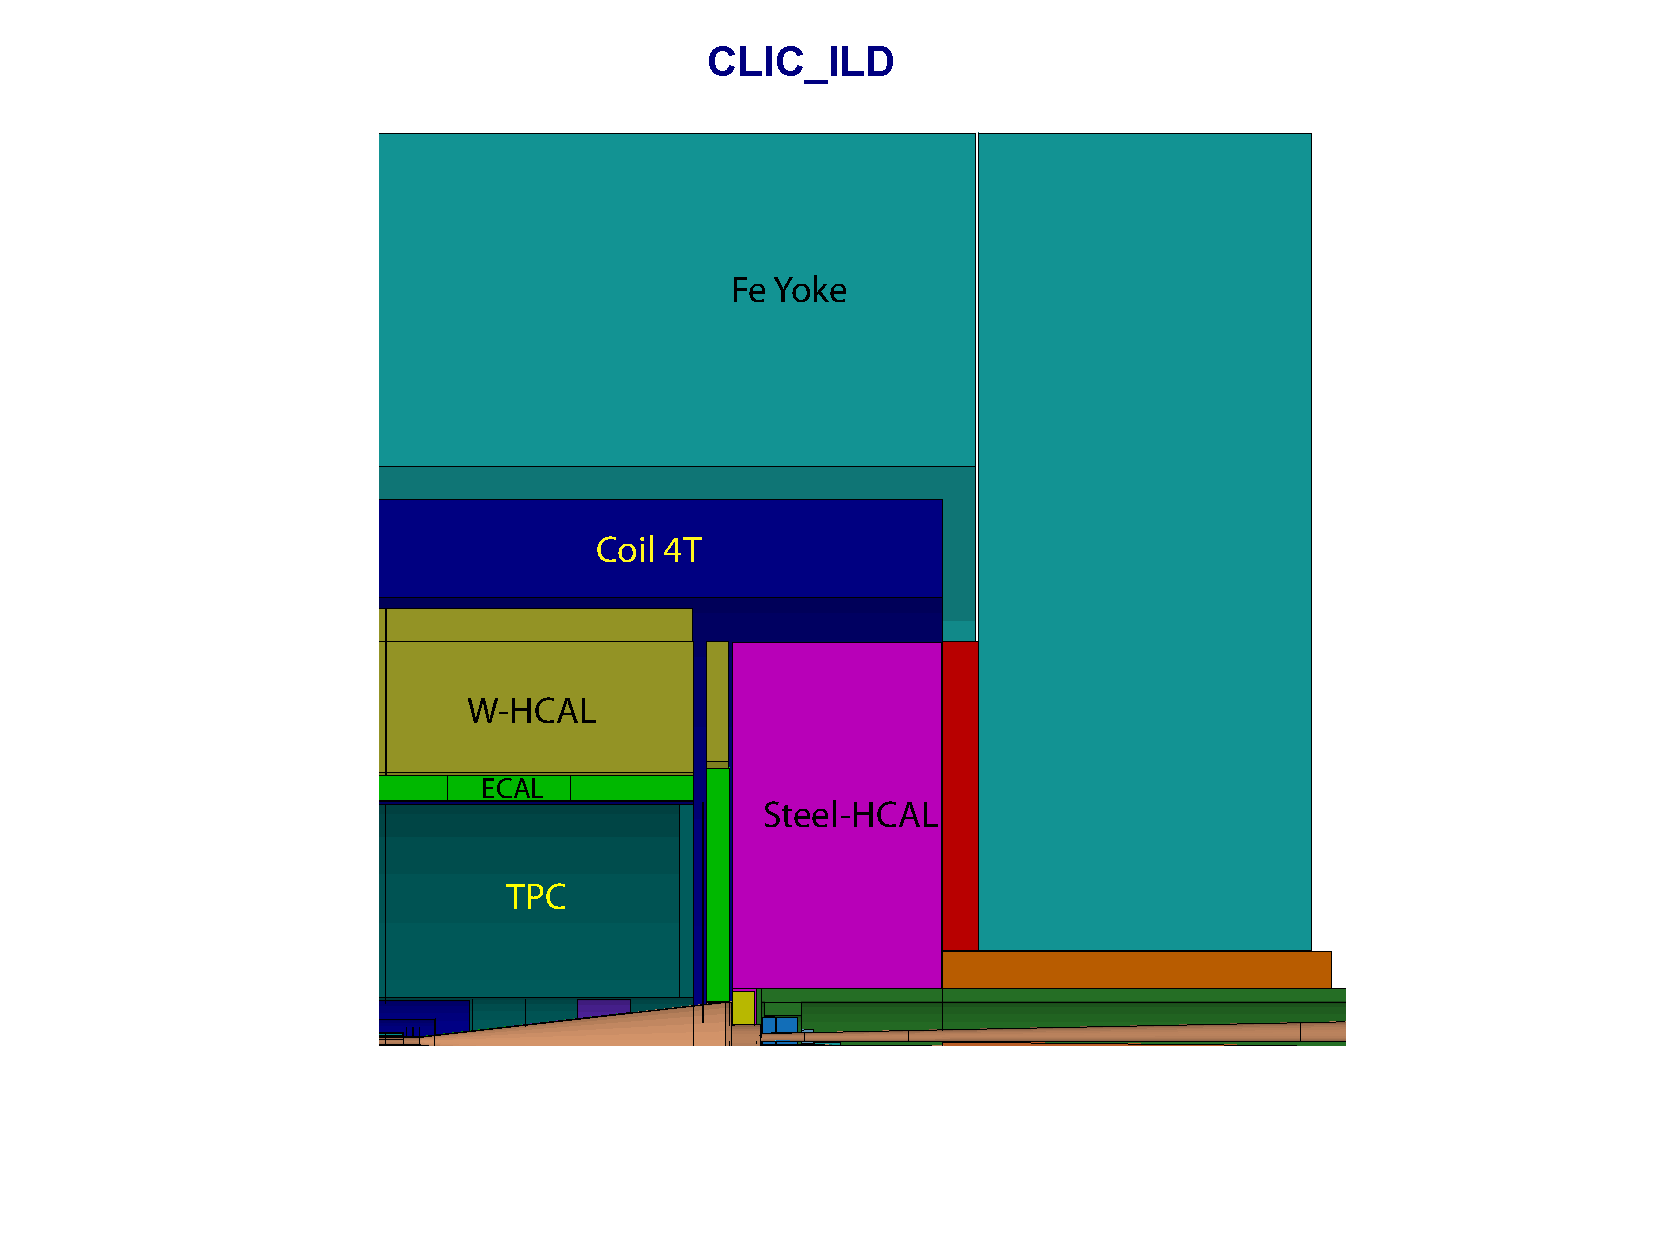
\includegraphics[width=5.5cm]{./CLIC_ILD_xz_box_view1.pdf}
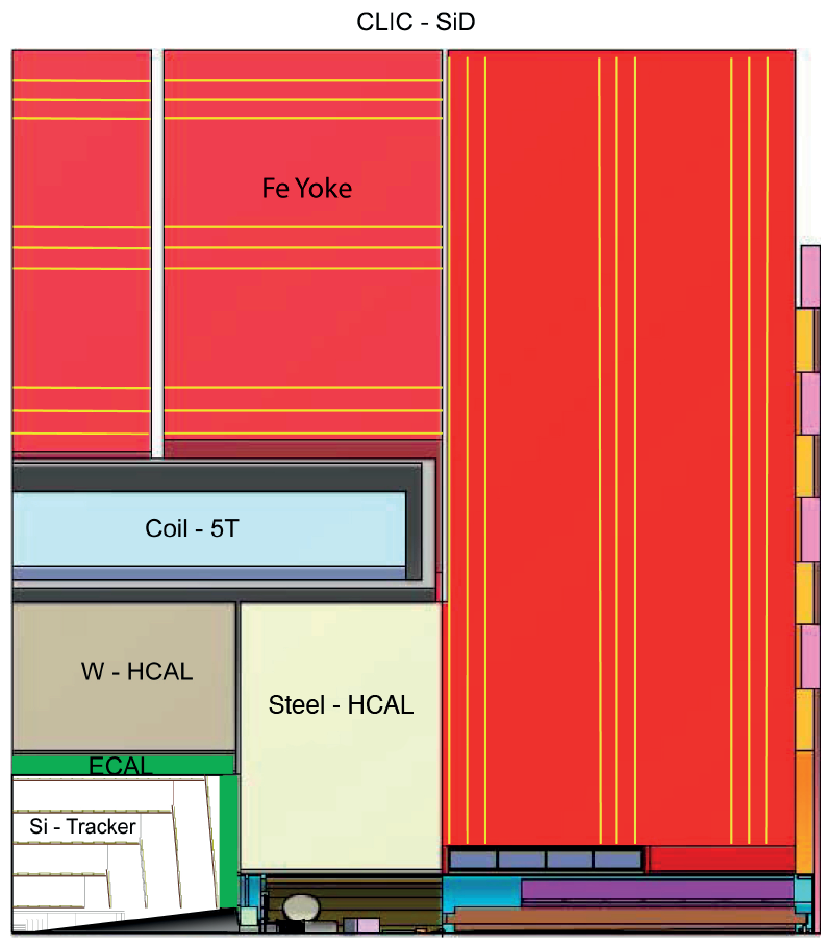
\includegraphics[width=5cm]{./CLIC_SiD_xz.pdf}
\end{center}
\end{frame}

\section{Samples considered}
\begin{frame}
\frametitle{Physics channels studied}
6 benchmark channels to assess detector performance:
\begin{itemize}
\item $\Pep\Pem \to \Ph \Pgne \Pagne, \Ph \to \mu^+\mu^-, \Ph \to
\Pbottom\APbottom$,
\item  $\Pep\Pem \to \PHp \PHm$, $\Pep\Pem \to \PHz \PA$, 
\item $\Pep\Pem \to \PSq_R \PaSq_R$, 
\item $\Pep\Pem \to \PSl \PaSl \,(\ell = \Pe,\Pgm,\Pgne)$, 
\item $\Pep\Pem \to \PSgxpm_i \PSgxmp_j,\, \Pep\Pem \to \PSgxz_i \PSgxz_j$,
\item  $\Pep\Pem \to \Pqt \Paqt$ (500~GeV).
\end{itemize}
2 different SUSY models, 2 different energies (luminosity spectra), many
background samples (SUSY and SM), millions of events needed
\end{frame}
%\begin{frame}
%\frametitle{Examples of results}
%\begin{center}
%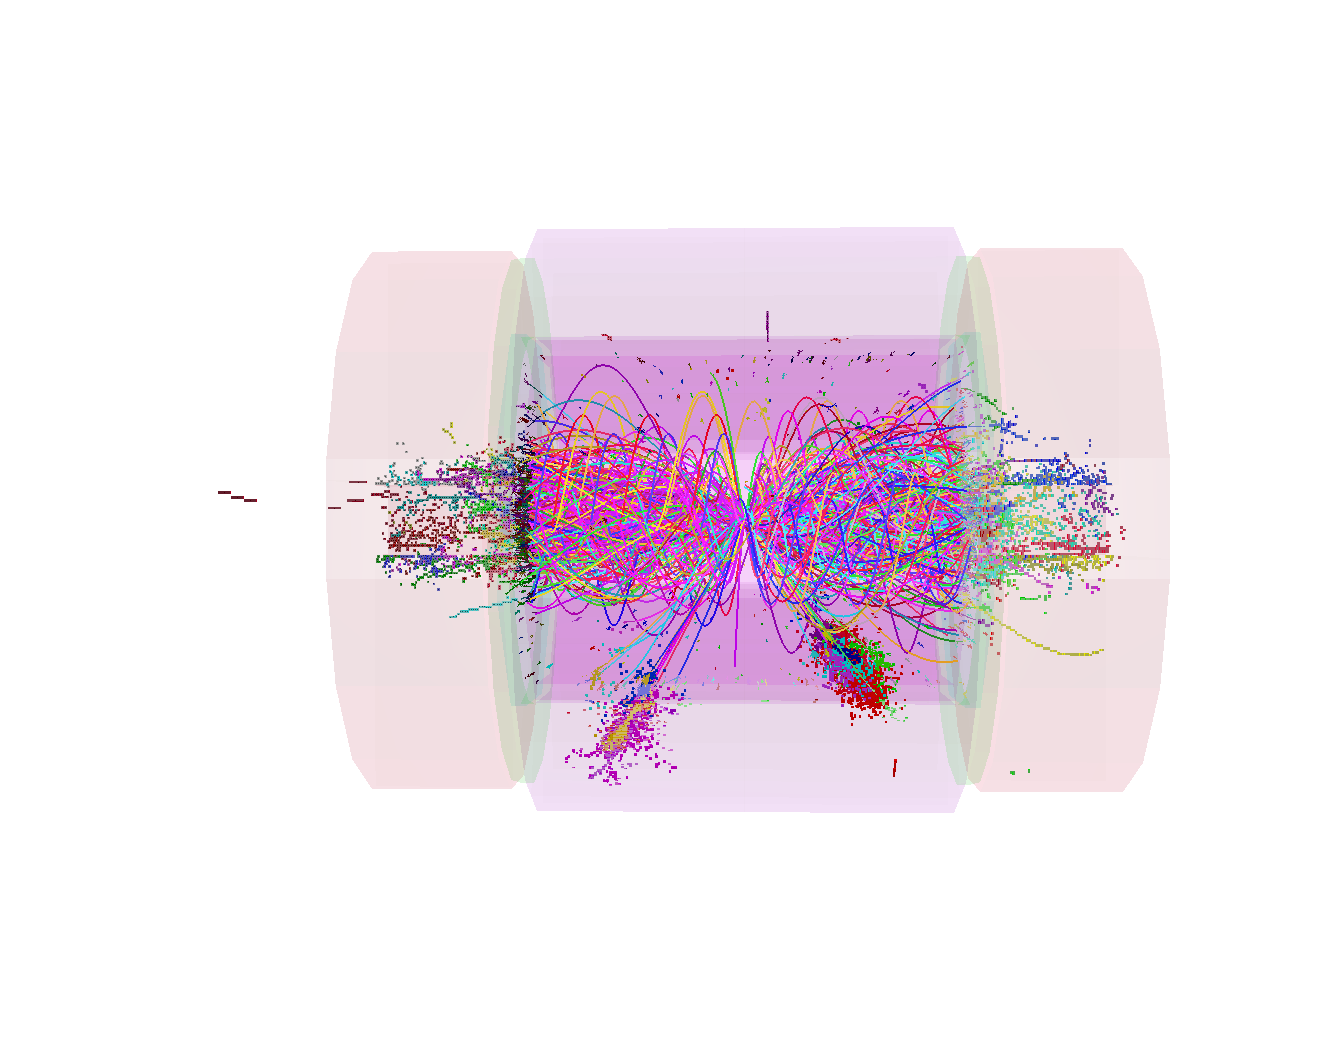
\includegraphics[width=6cm]{Squark2All}
%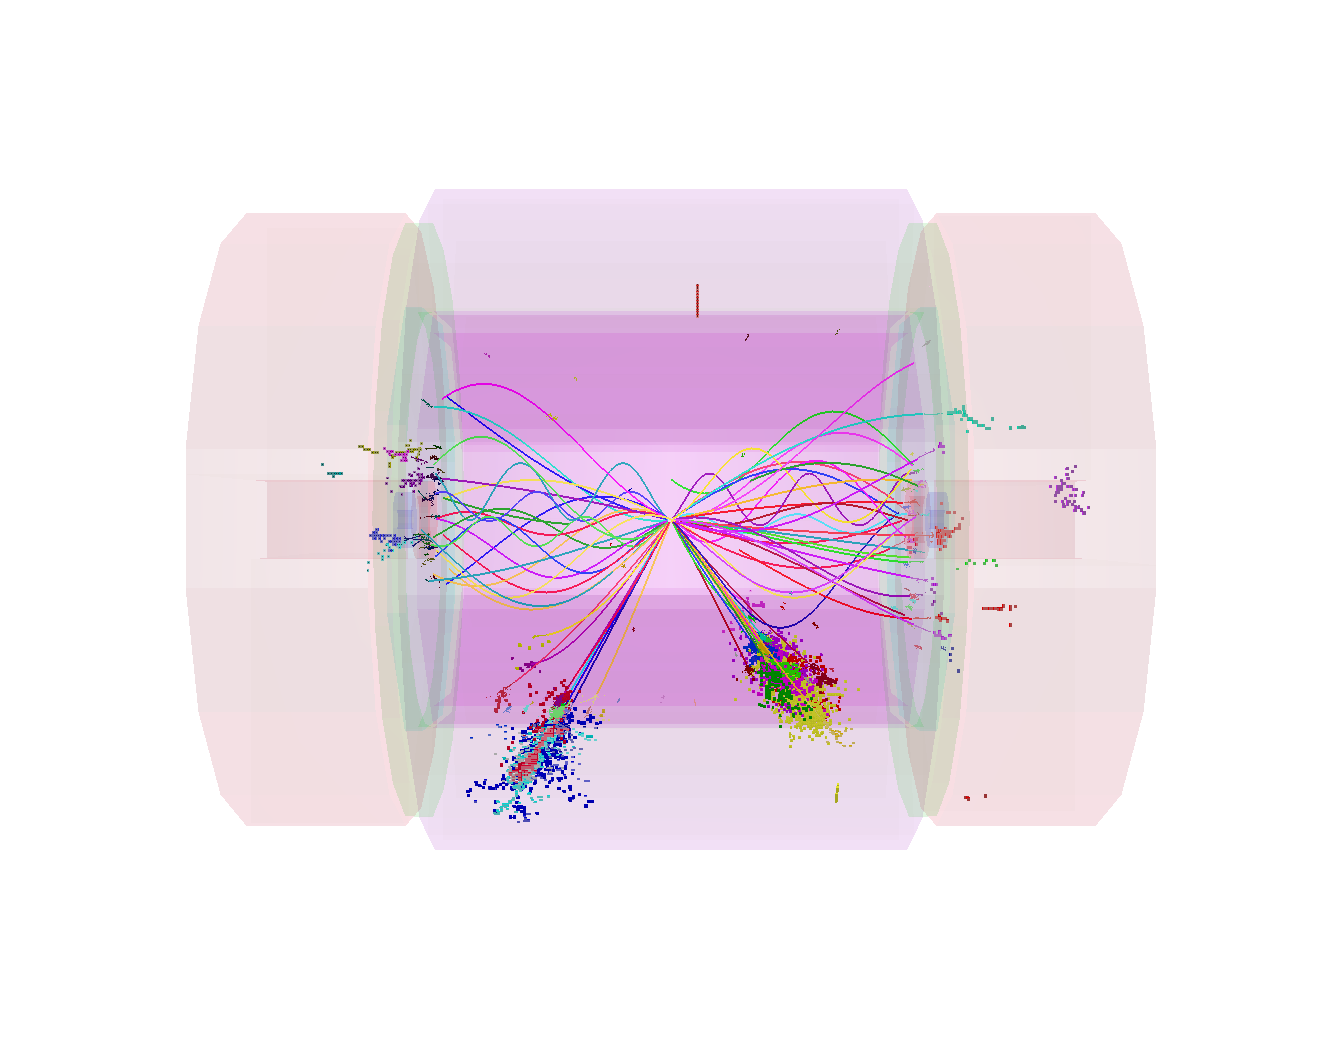
\includegraphics[width=6cm]{Squark2tight}
%\end{center}
%\end{frame}

\begin{frame}
\frametitle{Examples of results}
\begin{center}
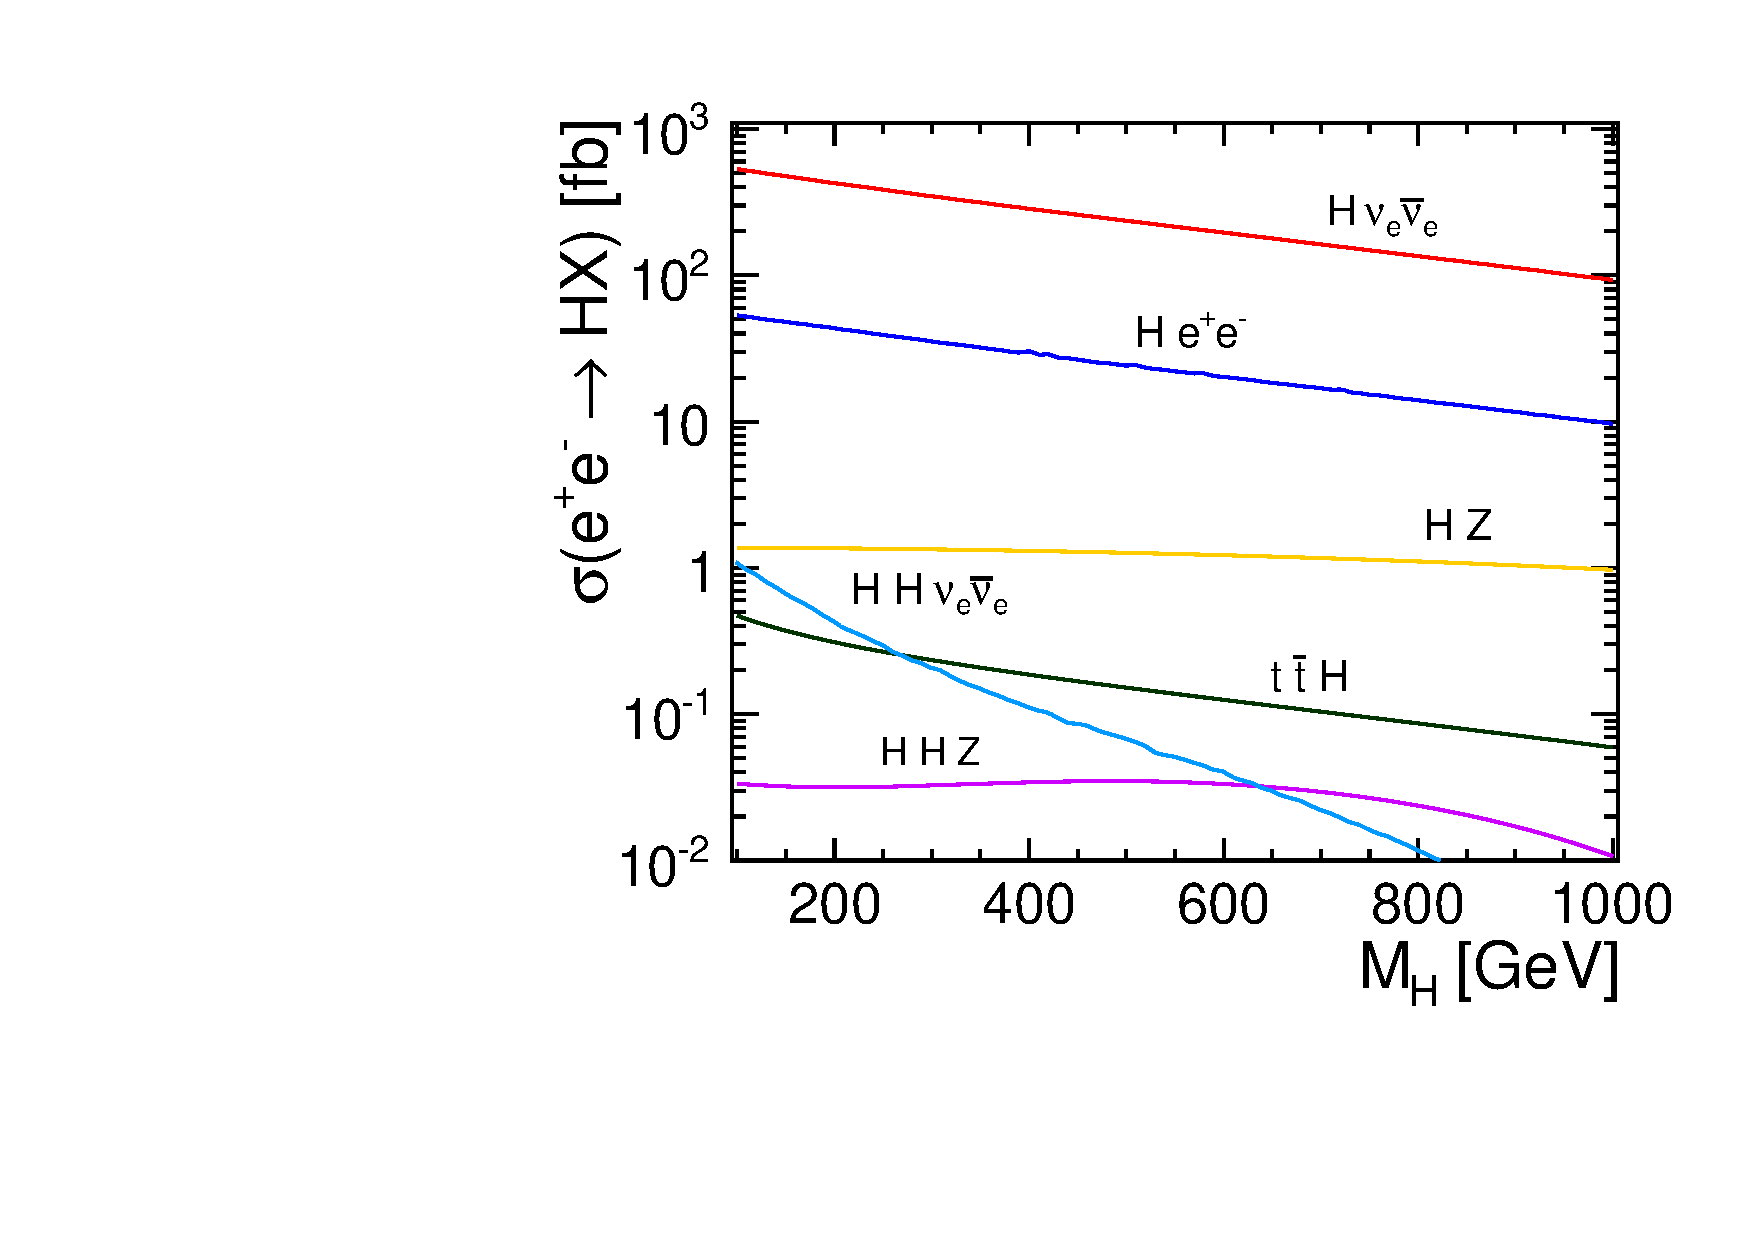
\includegraphics[width=5cm]{./xsec_vs_Hmass_sqrts3000.pdf}
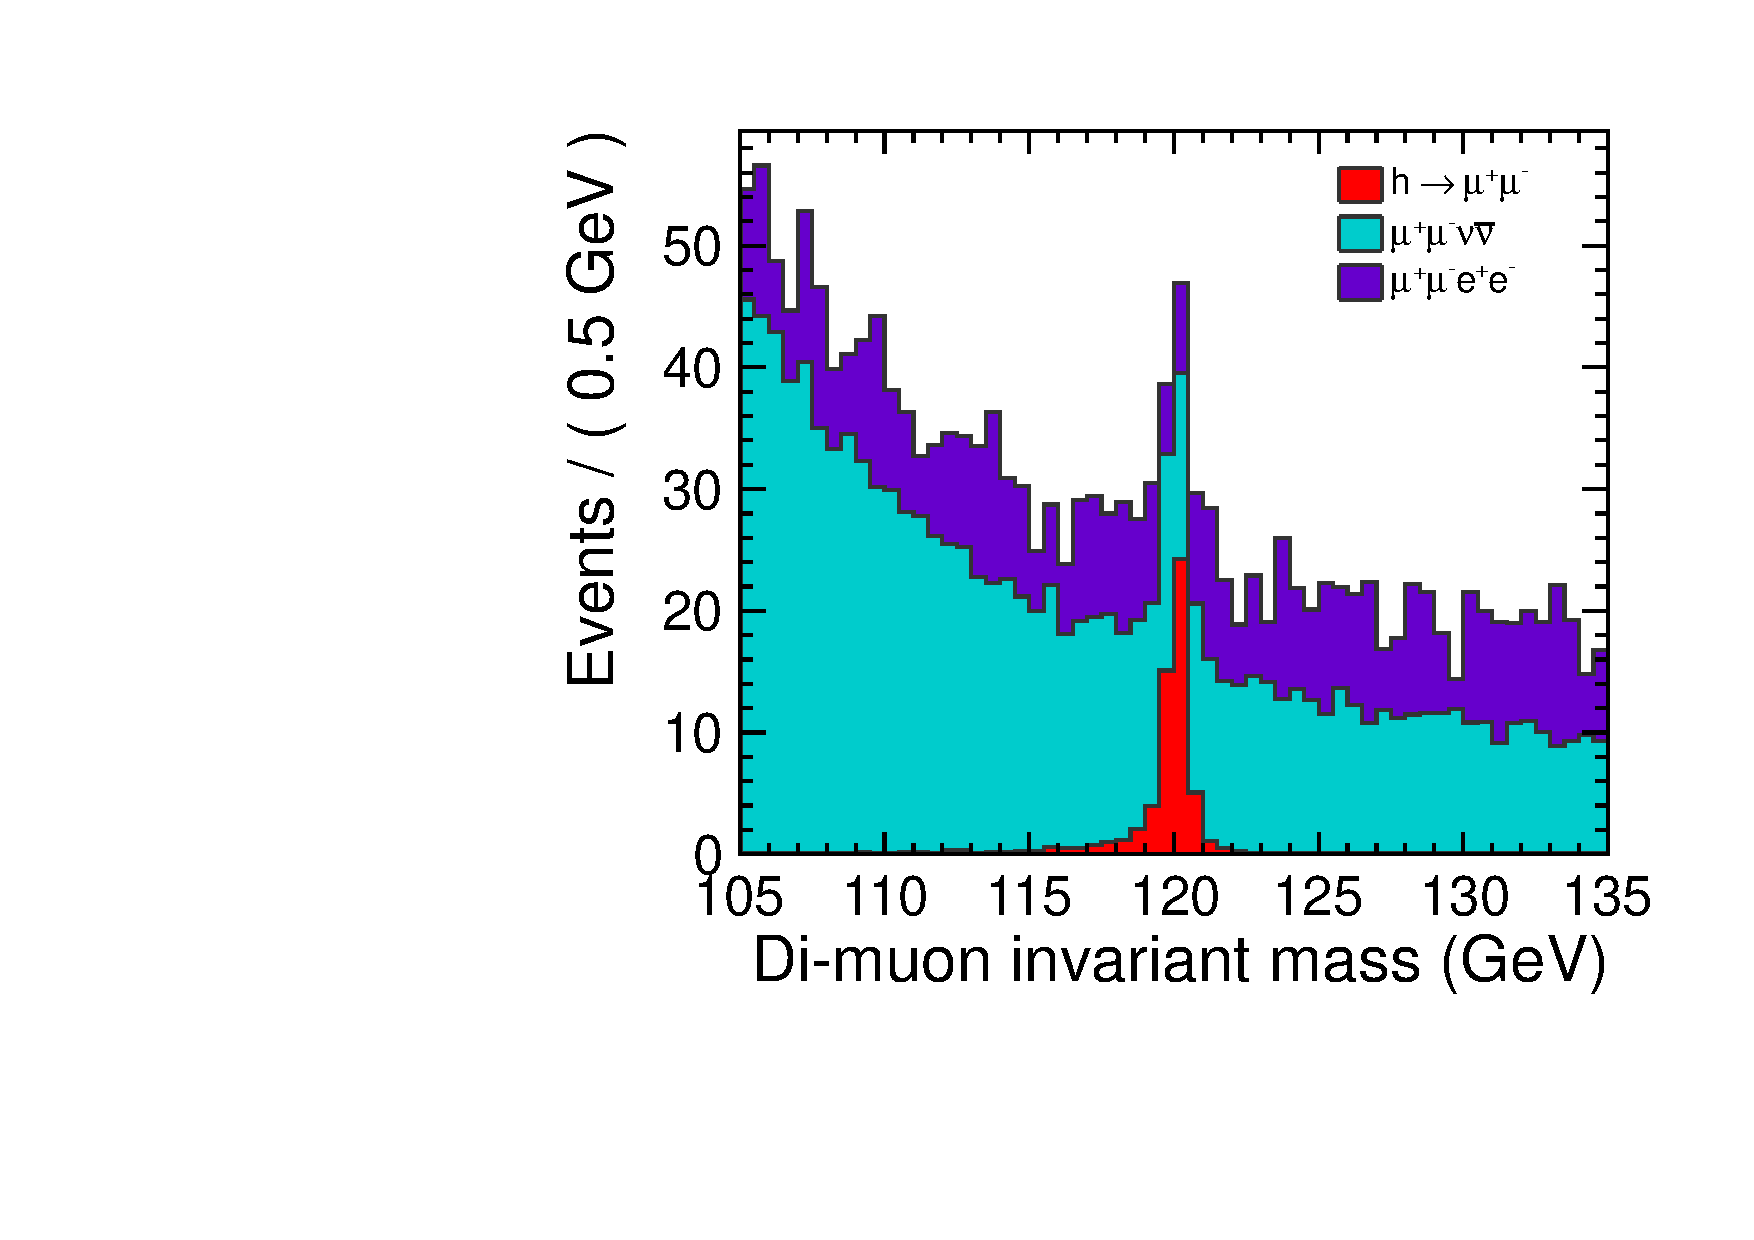
\includegraphics[width=5cm]{./ee_h_mumu_mass_mh120GeV.pdf}\\
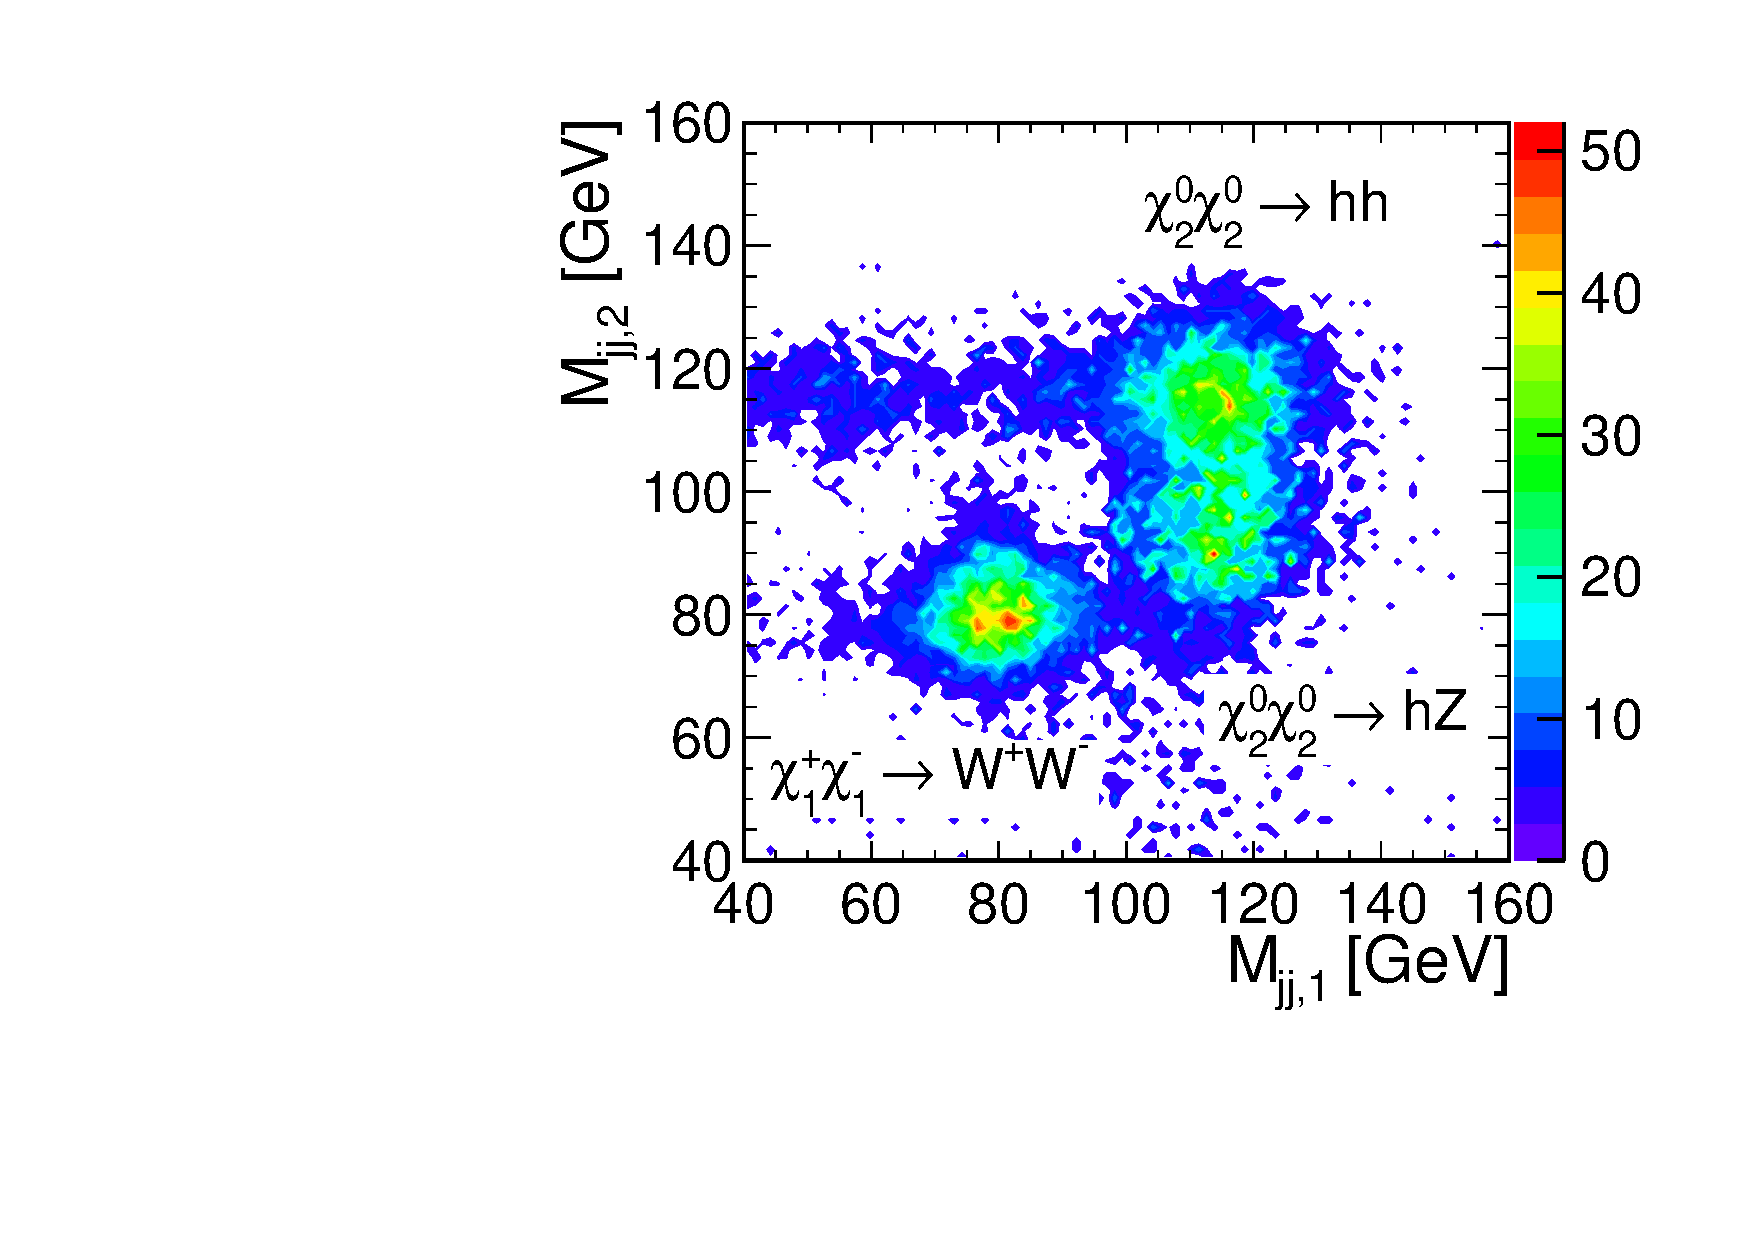
\includegraphics[width=5cm]{./MassPlot2D.pdf}
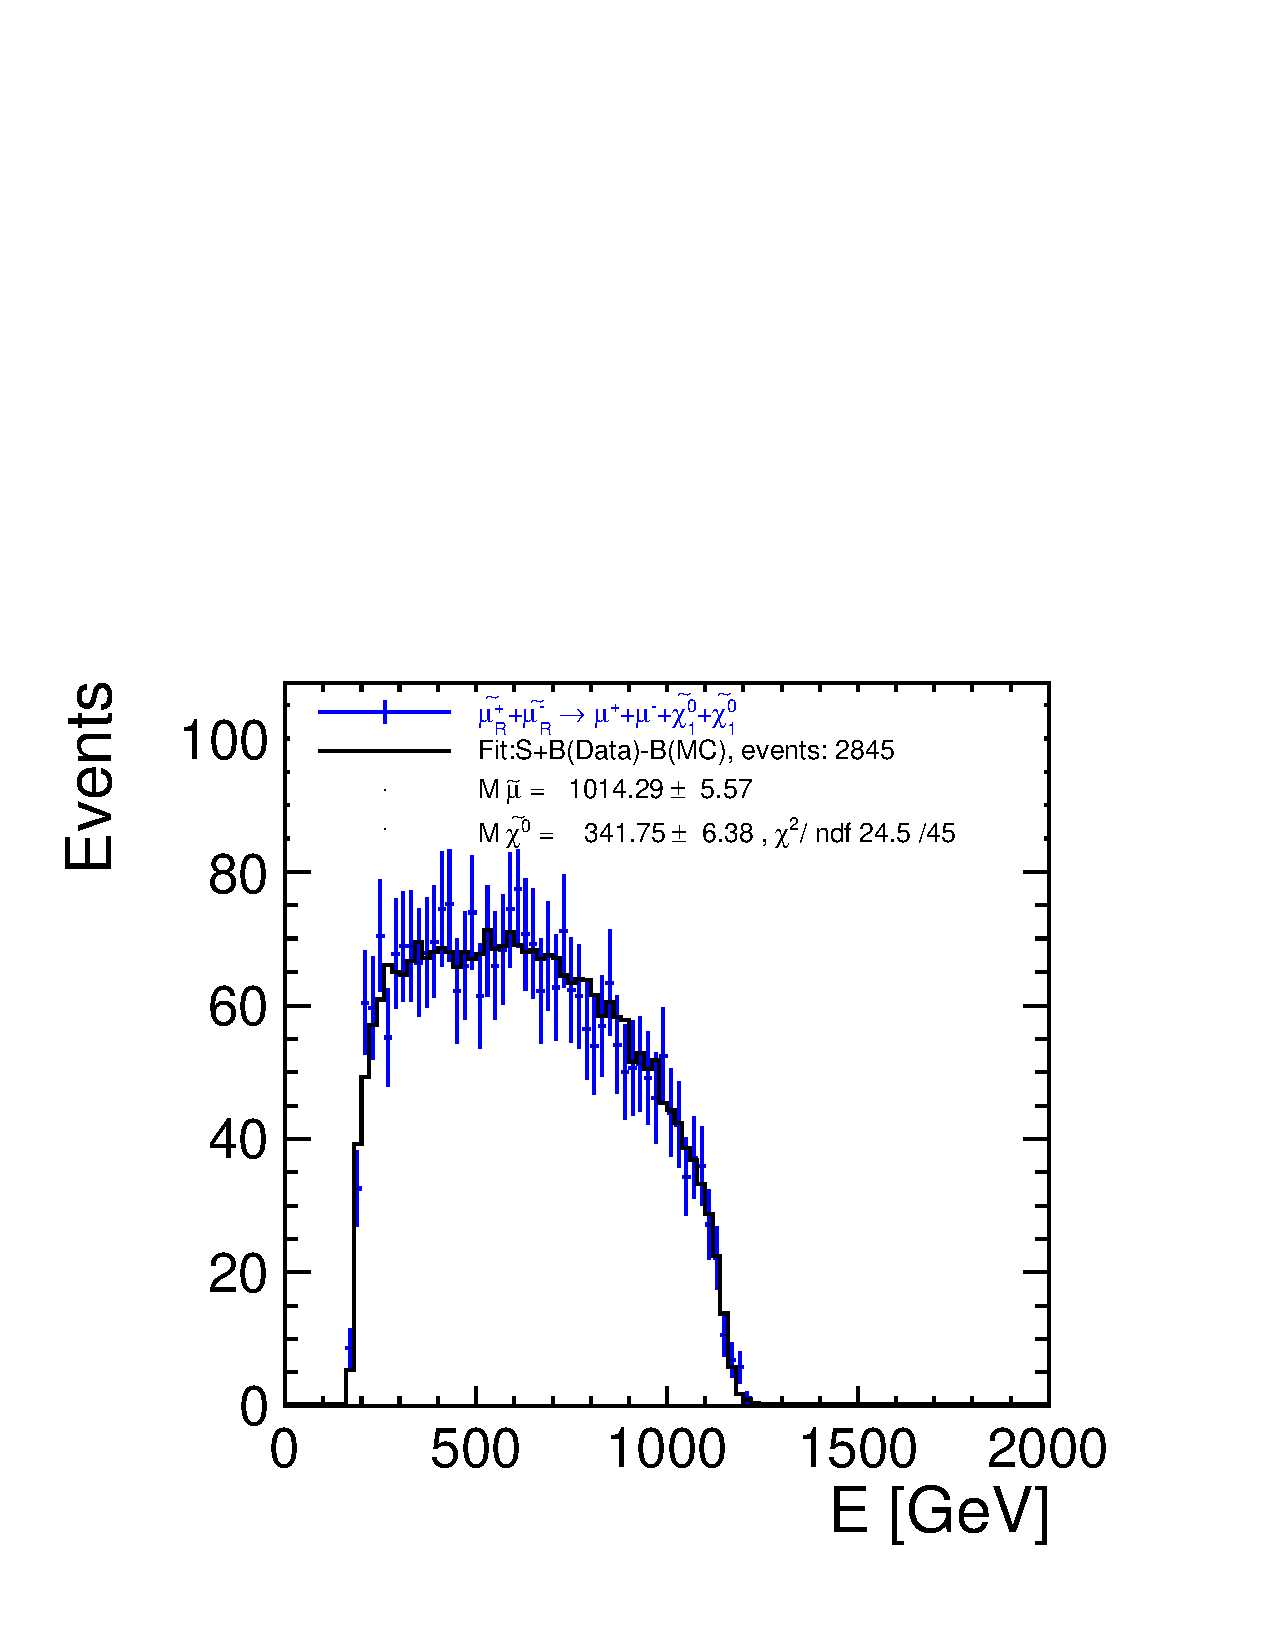
\includegraphics[width=5cm]{./205_H1LPADC4.pdf}
\end{center}
\end{frame}

\section{Modifications needed and Tools developed}
\begin{frame}
\frametitle{Modifications needed}
ILC LOIs used \whizard.\\
~\\
Several tweaks implemented (T.~Barklow, M.~Berggren, A.~Miyamoto):
\begin{itemize}
  \item Installation tools
  \item Specific support for luminosity spectra: chose between ILC, CLIC, etc.
  \item TAUOLA support
  \item Stdhep output
  \item 6 fermions final state handling (for ILC LOIs): $\Ptop\APtop$
  reconstruction
  \item Color flow (for DBD studies)
\end{itemize}
\end{frame}

\begin{frame}
\frametitle{Production framework}
CLIC detector studies use the {\color{blue} GRID} for mass production.\\
Need to  run many applications in heterogeneous context: \alert{ILCDIRAC}
\begin{itemize}
  \item Based on DIRAC: grid solution developed initially for the LHCb
  experiment. {\color{blue}PYTHON} based.
  \item Comes with production system: define task and let the system create
  and monitor the jobs.
\end{itemize}
~\\
Needed to interface \whizard in ILCDIRAC:
\begin{itemize}
  \item Run configuration: ILCDIRAC configuration is in PYTHON $\to$ convert to
  whizard.in
  \item Process selection: Make sure all relevant files (e.g. LesHouches files)
  are available
\end{itemize}
\end{frame}
\begin{frame}
\frametitle{Example of job definition}
\lstinputlisting[language=python,basicstyle=\scriptsize]{./WhizardExample.py}
Defines the \whizard executable to install.
\end{frame}
\begin{frame}
\frametitle{What happens on the grid node}
\begin{enumerate}
  \item Install software if not available
  \item Get files: user whizard.in, LesHouches file
  \item Set whizard.in as needed
  \item Set the environment: read the lumi spectra, set the library path
  \item Run \whizard
  \item Treat output: rename according to user convention and upload to Storage
  Element
\end{enumerate}
\end{frame}
\begin{frame}
\frametitle{Running \whizard in ILCDIRAC}
Problem: How to prevent users from trying non-existent channels?
\begin{itemize}
  \item Store the content of the whizard.prc in a file that can be used at
  submission time by DIRAC
  \item Keep relation between \whizard version and channels (SM vs SUSY)
\end{itemize}
~\\
Problem: How to reduce configuration issues?
\begin{itemize}
  \item Catch all errors before the job is submitted	
  \item New functionality: all \whizard options are wrapped in a
  XML file, also holds default values and types
\end{itemize}
\end{frame}

\begin{frame}
\frametitle{Running \whizard in the production for the CLIC CDR}
\begin{itemize}
  \item Framework is global: generation, simulation and reconstruction of events
  done using same tool (ILCDIRAC)
  \item Account for simulation/reconstruction CPU time constraints on the GRID
  (24 hours max on average)
  \item Account for optimal file sizes: Storage Element access is the most
  problematic
\end{itemize}
$\Rightarrow$ \alert{need to generate $10-1000$ events per job} depending on the
channel.
\end{frame}
\section{Limitations met}
\begin{frame}
\frametitle{Limitations met}
\begin{itemize}
  \item Impossible to generate specific final states with width: $\Ptop\APtop$,
  WW, ZZ, HH, HA. {\color{blue}Used PYTHIA standalone} for those. For SM Higgs
  processes assume width to be 0.\\
  ~\\
  \item Would have been useful to be able to {\color{blue}disable diagrams
  explicitly} to have pure signal samples\\
  ~\\
  \item Generator level cut interface not easily generalized: had to
  {\color{blue}add extra filtering programs} to run after \whizard.\\
  ~\\
  \item Process selection for people not compiling \whizard: Adding a
  {\color{blue}new process requires compiling a \whizard executable}, not easy
  from scratch
\end{itemize}
\end{frame}
\section{The future}
\begin{frame}
\frametitle{Using \whizard 2.0}
Using analysis framework of \whizard2:
\begin{center}
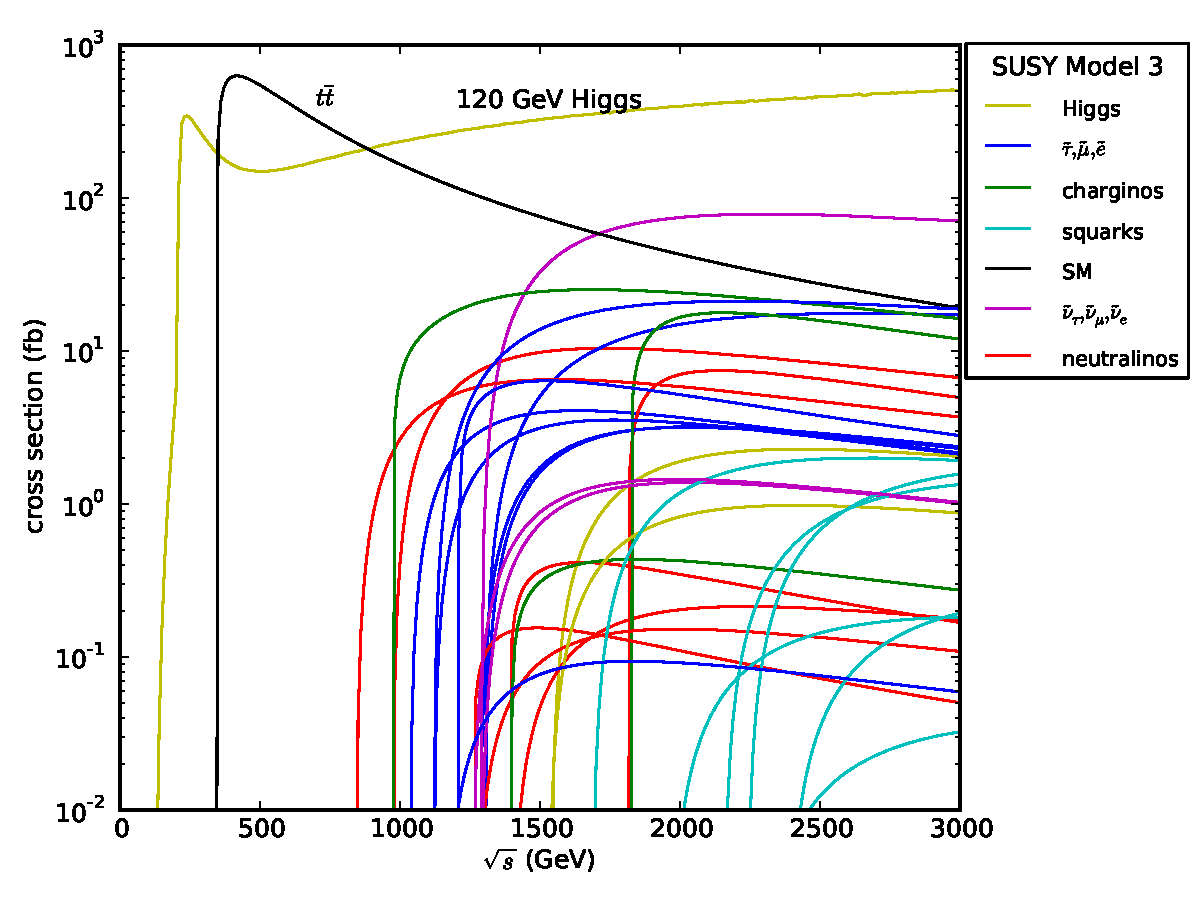
\includegraphics[width=7cm]{./model3.pdf}
\end{center}
Includes CLIC 3TeV luminosity spectrum.
\end{frame}
\section{Conclusion}
\begin{frame}
\frametitle{Conclusion}
For the CDR:
\begin{itemize}
  \item Very complete software
  \item Accurate cross sections
  \item Efficient event generation
  \item Lightweight to run on the GRID once compiled
  \item Compilation is tricky
  \item Some channels could not be done ($\Ptop\APtop$, WW, ZZ, HH, HA)
\end{itemize}
For \whizard 2.0:
\begin{itemize}
  \item Easier process selection
  \item Work on run configuration
  \item 8 fermions final states (ILC DBD studies)
\end{itemize}
\end{frame}
\begin{frame}
\frametitle{Conclusion} 
CDR has been internally reviewed, visible here:\\
 \url{https://edms.cern.ch/document/1160419}\\
~\\
Join the signatories here:\\
\url{https://indico.cern.ch/conferenceDisplay.py?confId=136364}
\end{frame}

\appendix
\begin{frame} 
\frametitle{Backup slides}
\end{frame}
\begin{frame}
\frametitle{Requests for the future}
\begin{itemize}
  \item Mechanism to suppress explicit contributions in processes
  \item Do not depend on compiler at run time (More or less OK if I understand)
  \item Interface to other languages (e.g. XML, PYTHON)
\end{itemize}
\end{frame}
\begin{frame}
\frametitle{Making \whizard2.0 and ILCDIRAC play well with each other}
\begin{itemize}
  \item Install \whizard2.0 on an ILCDIRAC server
  \item Interface properly in ILCDIRAC (.sin content)
  \item Make the central installation compile the process on the fly (Request
  mechanism)
  \item Register that \whizard version as a new application and install it on
  the sites
  \item Run the user job against this version when compilation is done
\end{itemize}
Needs to hold on some database the processes (can use some checksum mechanism)
and the versions.
\end{frame}
\end{document}
